\documentclass[11pt, a4paper]{article}

\usepackage[top=2cm, bottom=2cm, left=2.5cm, right=2cm]{geometry}
\usepackage{fontspec}
\usepackage{amsmath, amssymb}
\usepackage{booktabs}
\usepackage{tabularx}
\usepackage{array}
\usepackage{graphicx}
\usepackage{float}
\usepackage{xcolor}
\usepackage{hyperref}
\usepackage{xurl}
\usepackage{parskip}
\usepackage{microtype}
\usepackage{caption}
\usepackage{enumitem}
\usepackage{tikz}

\graphicspath{{images/}}
\emergencystretch=10em

\hypersetup{
    colorlinks=true,
    linkcolor=blue!70!black,
    citecolor=blue!70!black,
    urlcolor=blue!70!black,
    pdftitle={Assignment 06 - Recurrent Neural Networks: scratch, Keras and PyTorch},
    pdfauthor={Luu Anh Dung}
}

\newcommand{\run}[1]{\texttt{#1}}
\setlist{itemsep=2pt, topsep=4pt}

\begin{document}

% ---------------------------------------------------------
% COVER PAGE
% ---------------------------------------------------------
\begin{titlepage}
\begin{center}
\vspace*{0.5cm}
\Large
\textbf{POSTS AND TELECOMMUNICATIONS INSTITUTE OF TECHNOLOGY}\\
\textbf{Faculty of Information Technology}

\vspace{2.0cm}
\Huge
\textbf{Intelligent System Development}\\
\vspace{0.4cm}
\LARGE
\textbf{ASSIGNMENT 06}\\
\vspace{0.6cm}
\Large
\textbf{Recurrent Neural Networks on Time Series:\\From Scratch, in Keras and in PyTorch}

\vfill
\normalsize
\begin{tabular}{rl}
\textbf{Instructor / Lecturer:} & Assoc. Prof. Dinh Que Tran, Ph.D. \\
\textbf{Email:} & quetd@ptit.edu.vn, tdque@yahoo.com \\[0.8cm]
\textbf{Student Name:} & Lưu Anh Dũng \\
\textbf{Student ID:} & B23DCDK036 \\
\textbf{Semester:} & I.2025 -- 2026 \\
\textbf{Submission:} & Individual Project \\
\end{tabular}

\vfill
\textbf{Hanoi, 2026}
\vspace{0.5cm}
\end{center}
\end{titlepage}

\tableofcontents
\newpage

% =====================================================================
\section{Overview}
% =====================================================================

This report studies the recurrent neural network (RNN) and implements the same model three times: \textbf{from scratch} in NumPy (\run{SC}: hand-written
forward pass, back-propagation through time and Adam), in \textbf{Keras} (\run{TF}) and in \textbf{PyTorch} (\run{PT}). It is applied to two time-related
datasets from Kaggle, each between 100 and 150\,MB:
\begin{itemize}
\item \textbf{EC — a service process in e-commerce.} The Olist marketplace (Brazil, 2016--2018): from the last 10 orders sent to the same state,
  predict how many days the newest order will take to be delivered (96{,}227 windows).
\item \textbf{ST — stock prices.} 250 NYSE stocks (2010--2016): from the last 30 trading days, predict the next day's trading range, a measure of risk
  (432{,}750 windows).
\end{itemize}
Both tasks are many-to-one regression. All implementations share the data, the split, the architecture (one vanilla RNN layer with 32 units and a
linear head), the starting weights, the optimizer, the early-stopping rule and the hardware (CPU), so only the abstraction level changes.
LSTM and GRU are added in Keras and PyTorch. Run IDs have the form \run{<dataset>-<implementation>-<model>}, e.g.\ \run{ST-TF-GRU}.

\begin{table}[H]
\centering
\caption{All 14 runs, test period. RMSE in days (EC, top) and in percentage points of daily range (ST, bottom); $R^2$ is out-of-sample against the
train mean; s/epoch = median time per epoch on CPU.}
\label{tab:summary}
\small
\begin{tabular}{lrrrr}
\toprule
Run & test RMSE & $R^2$ & params & s/epoch \\
\midrule
\run{EC-SC-RNN} & 5.014 d & 0.543 & 1{,}409 & 0.2 \\
\run{EC-TF-RNN} & 4.968 d & 0.557 & 1{,}409 & 0.6 \\
\run{EC-PT-RNN} & 4.916 d & 0.549 & 1{,}409 & 0.8 \\
\run{EC-TF-LSTM} & 4.916 d & 0.563 & 5{,}537 & 1.3 \\
\run{EC-PT-LSTM} & 4.829 d & 0.573 & 5{,}665 & 1.8 \\
\run{EC-TF-GRU} & 4.869 d & 0.579 & 4{,}257 & 1.5 \\
\run{EC-PT-GRU} & 4.821 d & 0.574 & 4{,}257 & 1.5 \\
\midrule
\run{ST-SC-RNN} & 1.1897 pp & 0.522 & 1{,}313 & 2.3 \\
\run{ST-TF-RNN} & 1.1894 pp & 0.529 & 1{,}313 & 5.5 \\
\run{ST-PT-RNN} & 1.1842 pp & 0.529 & 1{,}313 & 8.0 \\
\run{ST-TF-LSTM} & 1.1559 pp & 0.537 & 5{,}153 & 14.8 \\
\run{ST-PT-LSTM} & 1.1454 pp & 0.534 & 5{,}281 & 22.1 \\
\run{ST-TF-GRU} & 1.1606 pp & 0.537 & 3{,}969 & 17.3 \\
\run{ST-PT-GRU} & 1.1486 pp & 0.533 & 3{,}969 & 17.9 \\
\bottomrule
\end{tabular}
\end{table}

\textbf{Key takeaways}
\begin{enumerate}
\item \textbf{The three implementations compute the same function.} With identical weights the forward passes differ by less than $5\cdot10^{-7}$ and
  the parameter counts are equal (1{,}409 for EC, 1{,}313 for ST). After training the core RNN ends within 2\,\% (EC) and 0.5\,\% (ST) across implementations;
  the spread comes from batch order and the stopping epoch, not from the mathematics.
\item \textbf{On EC the sequence helps.} Every recurrent model beats every baseline: RMSE 4.82--5.01 days against 5.22 for last week's mean delivery time
  to the state, 5.26 for a linear model on the same inputs and 5.41 for Olist's recalibrated promise ($R^2$ 0.54--0.58 vs.\ at most 0.48).
\item \textbf{On ST risk is predictable, but the classic linear HAR model is as good.} The RNNs reach $R^2=0.52$--$0.54$ and call the direction of
  tomorrow's change in risk correctly 70.5--71.1\,\% of the time, far above naive forecasts; the best (PyTorch LSTM) only ties HAR (1.1454 vs.\ 1.1449 pp).
\item \textbf{Gates help moderately.} LSTM/GRU are the best models on both datasets (1--3\,\% lower RMSE than the vanilla RNN), at 2--3$\times$ the time per epoch
  and 3--4$\times$ the parameters. The vanilla RNN passes only 2\,\% (EC) and 6\,\% (ST) of the learning signal to the oldest step of its window.
\item \textbf{Cost.} For the vanilla RNN on CPU the NumPy loop is the fastest per epoch (EC 0.24\,s, ST 2.3\,s) ahead of Keras (0.6, 5.5\,s) and PyTorch (0.8, 8.0\,s),
  because the model is tiny and the frameworks carry fixed overhead per batch.
\end{enumerate}

% =====================================================================
\section{Theoretical Background of Recurrent Networks}
% =====================================================================

This chapter develops what is needed to read the rest of the report: the forecasting task (\ref{sec:task}), the operators (\ref{sec:ops}), the recurrent cell
(\ref{sec:cell}), training (\ref{sec:train}), vanishing and exploding gradients (\ref{sec:vanish}), gated cells (\ref{sec:gates}), evaluation (\ref{sec:eval}) and the
same layer in three libraries (\ref{sec:three}). Every numeric example was checked in the concepts notebook against NumPy, finite differences or PyTorch.
Notation: $N$ windows, $T$ window length, $F$ features per step, $H$ hidden size; $x_t\in\mathbb{R}^F$, $h_t\in\mathbb{R}^H$, prediction $\hat y$, target $y$, loss $L$.
Vectors are row vectors, so a layer is written $xW$.

\subsection{Sequences and the Forecasting Problem}
\label{sec:task}

\textbf{Order is information.} A dense network sees one vector and has no notion of which input came first. In a sequence the order matters: delivery times
of 8, 12, 15 days (logistics getting worse) and 15, 12, 8 (recovering) have the same mean but call for different forecasts.

\textbf{Windows.} A series $s_1,\dots,s_n$ becomes supervised pairs by sliding a window of $T$ steps: input $(s_k,\dots,s_{k+T-1})$, target $s_{k+T}$.
For the delivery times $8,12,9,15,7,21,10$ and $T=3$: $[8,12,9]\to15$, $[12,9,15]\to7$, $[9,15,7]\to21$, $[15,7,21]\to10$. Stacked, inputs form a tensor
$X\in\mathbb{R}^{N\times T\times F}$ — here $(4,3,1)$; in the EC experiment $(96\text{k},10,10)$, in ST $(433\text{k},30,7)$. Windows of many series (states, stocks) are stacked
along $N$ so that one model serves all of them.

\textbf{Task shapes.} \emph{Many-to-one} reads $T$ steps and outputs one value from the last state (used here); \emph{many-to-many} outputs at every step; \emph{one-to-many}
generates a sequence. Only which states feed the output layer changes.

\textbf{Time order in evaluation.} The data are split in time: train on the past, validate and test on the future, and fit scaling statistics on the train period only.
A random split would let the model learn from days after the ones it is tested on.

\subsection{Mathematical Operators}
\label{sec:ops}

\begin{itemize}
\item \textbf{Matrix product} $(xW)_j=\sum_ix_iW_{ij}$ mixes inputs and memory into $H$ new values: $(2,1)\begin{pmatrix}1&-1\\0.5&2\end{pmatrix}=(2.5,\,0)$.
\item \textbf{Bias} shifts each unit: $(2.5,0)+(-0.5,0.1)=(2,0.1)$.
\item \textbf{Hyperbolic tangent} $\tanh z\in(-1,1)$, $\tanh'(z)=1-\tanh^2 z$: $\tanh 2=0.964$ and $\tanh'(2)=0.071$ — a saturated unit passes 7\,\% of a gradient.
\item \textbf{Sigmoid} $\sigma(z)=1/(1+e^{-z})\in(0,1)$, $\sigma'=\sigma(1-\sigma)\le0.25$; used for gates: $\sigma(3)=0.953$.
\item \textbf{Element-wise (Hadamard) product} $(a\odot b)_i=a_ib_i$ applies a gate to a value: $(0.95,0.1)\odot(2,2)=(1.9,0.2)$.
\item \textbf{Softmax} $e^{z_i}/\sum_je^{z_j}$ turns scores into probabilities, $(2,1,0)\mapsto(0.665,0.245,0.090)$; needed for classification, not for the regression heads used here.
\item \textbf{Concatenation.} $x_tW_{xh}+h_{t-1}W_{hh}=[x_t,h_{t-1}]\begin{bmatrix}W_{xh}\\W_{hh}\end{bmatrix}$: frameworks compute one larger product; the result is identical.
\end{itemize}

\subsection{The Recurrent Cell}
\label{sec:cell}

The network keeps a state $h_t\in\mathbb{R}^H$ that summarises everything read so far:
\begin{equation}
h_t=\tanh\big(x_tW_{xh}+h_{t-1}W_{hh}+b\big),\qquad h_0=0,\qquad \hat y=h_TW_{hy}+b_y,
\label{eq:rnn}
\end{equation}
with $W_{xh}\in\mathbb{R}^{F\times H}$, $W_{hh}\in\mathbb{R}^{H\times H}$, $b\in\mathbb{R}^H$, $W_{hy}\in\mathbb{R}^{H\times1}$. \emph{Unrolling} draws the loop as $T$ copies of one cell
(Figure~\ref{fig:unroll}). The copies \emph{share} their weights, so the parameter count $FH+H^2+H$ (cell) $+H+1$ (head) does not depend on $T$: the 10-step EC cell
and the 30-step ST cell have the same size for equal $F$.

\begin{figure}[H]
\centering
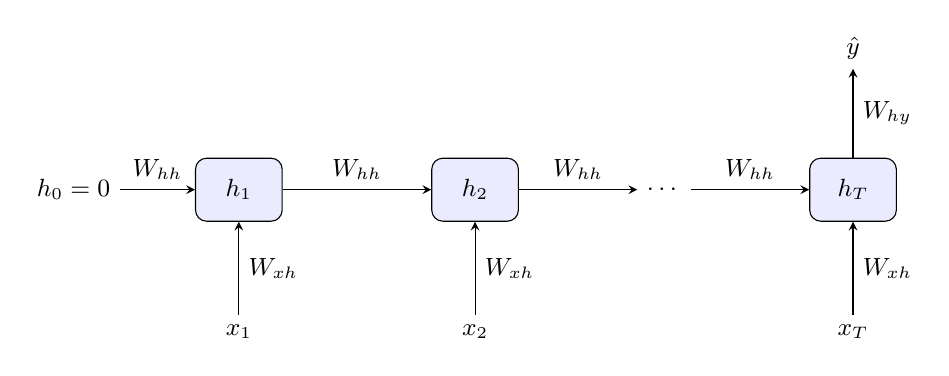
\begin{tikzpicture}[>=stealth, font=\small,
  cell/.style={draw, rounded corners, minimum width=1.1cm, minimum height=0.8cm, fill=blue!8}]
\node[cell] (h1) at (0,0) {$h_1$};
\node[cell] (h2) at (3,0) {$h_2$};
\node (d) at (5.4,0) {$\cdots$};
\node[cell] (hT) at (7.8,0) {$h_T$};
\node (h0) at (-2.1,0) {$h_0=0$};
\node (x1) at (0,-1.8) {$x_1$};
\node (x2) at (3,-1.8) {$x_2$};
\node (xT) at (7.8,-1.8) {$x_T$};
\node (y) at (7.8,1.8) {$\hat y$};
\draw[->] (h0) -- node[above]{$W_{hh}$} (h1);
\draw[->] (h1) -- node[above]{$W_{hh}$} (h2);
\draw[->] (h2) -- node[above]{$W_{hh}$} (d);
\draw[->] (d) -- node[above]{$W_{hh}$} (hT);
\draw[->] (x1) -- node[right]{$W_{xh}$} (h1);
\draw[->] (x2) -- node[right]{$W_{xh}$} (h2);
\draw[->] (xT) -- node[right]{$W_{xh}$} (hT);
\draw[->] (hT) -- node[right]{$W_{hy}$} (y);
\end{tikzpicture}
\caption{A many-to-one RNN unrolled over $T$ steps; the same $W_{xh}$, $W_{hh}$, $b$ are used at every step and only $h_T$ feeds the output.}
\label{fig:unroll}
\end{figure}

\textbf{Worked example} ($F=1$, $H=2$, $b=0$). Daily ranges $1.2, 1.1, 2.9\,\%$, centred by subtracting 1.5: $x=(-0.3,-0.4,1.4)$, with
$W_{xh}=(0.8,\,-0.5)$ and $W_{hh}=\begin{pmatrix}0.5&0\\0.2&0.3\end{pmatrix}$:

\begin{center}
\small
\begin{tabular}{cccc}
\toprule
$t$ & $x_t$ & $z_t=x_tW_{xh}+h_{t-1}W_{hh}$ & $h_t=\tanh z_t$ \\
\midrule
1 & $-0.3$ & $(-0.24,\ 0.15)$ & $(-0.2355,\ 0.1489)$ \\
2 & $-0.4$ & $(-0.4080,\ 0.2447)$ & $(-0.3867,\ 0.2399)$ \\
3 & $\phantom{-}1.4$ & $(0.9746,\ -0.6280)$ & $(0.7507,\ -0.5567)$ \\
\bottomrule
\end{tabular}
\end{center}
Unit~1 tracks ``risk is high now''; the two calm days still enter $z_3$ through $h_2W_{hh}$. PyTorch's \texttt{nn.RNN} with the same weights gives the same $h_3$ to $10^{-6}$.

\textbf{Memory.} For one unit in its near-linear range, a small input spike decays as $h_t\approx w^{t-1}h_1$ for recurrent weight $w$: with $w=0.9$ the spike keeps
$0.9^{9}=39\,\%$ after 10 steps, with $w=0.5$ only $0.2\,\%$ (Figure~\ref{fig:concepts}, left). The recurrent weight sets the memory length.

\subsection{Training a Recurrent Network}
\label{sec:train}

\textbf{Back-propagation through time (BPTT).} With $z_t=x_tW_{xh}+h_{t-1}W_{hh}+b$ and $L=\frac1N\sum(\hat y-y)^2$:
\begin{equation}
\frac{\partial L}{\partial h_T}=\tfrac2N(\hat y-y)W_{hy}^\top,\qquad
\frac{\partial L}{\partial z_t}=\frac{\partial L}{\partial h_t}\odot(1-h_t^2),\qquad
\frac{\partial L}{\partial h_{t-1}}=\frac{\partial L}{\partial z_t}W_{hh}^\top,
\label{eq:bptt}
\end{equation}
and each shared weight collects one contribution per step:
$\partial L/\partial W_{xh}=\sum_tx_t^\top\,\partial L/\partial z_t$, $\partial L/\partial W_{hh}=\sum_th_{t-1}^\top\,\partial L/\partial z_t$, $\partial L/\partial b=\sum_t\partial L/\partial z_t$.

\textbf{Scalar example.} $h_t=\tanh(wx_t+uh_{t-1})$, $\hat y=h_2$, $x=(1,0.5)$, $w=0.6$, $u=0.9$, $y=0$. Forward: $h_1=\tanh0.6=0.5370$, $h_2=\tanh(0.3+0.9\cdot0.5370)=0.6546$,
$L=0.4285$. Backward: $\partial L/\partial z_2=2\cdot0.6546\,(1-0.6546^2)=0.7482$; step-2 share of $\partial L/\partial u$ is $0.7482\cdot h_1=0.4018$, step~1 adds $0$ (since $h_0=0$);
$\partial L/\partial z_1=0.7482\cdot u\,(1-h_1^2)=0.4792$ and $\partial L/\partial w=0.7482\cdot0.5+0.4792\cdot1=0.8533$. PyTorch autograd returns the same 0.4018 and 0.8533.

\textbf{Adam} keeps running averages of the gradient and its square, $m\leftarrow\beta_1m+(1-\beta_1)g$, $v\leftarrow\beta_2v+(1-\beta_2)g^2$, and steps
$\theta\leftarrow\theta-\eta\,\hat m/(\sqrt{\hat v}+\epsilon)$ with bias-corrected $\hat m,\hat v$; $\beta_1=0.9$, $\beta_2=0.999$, $\eta=10^{-3}$, $\epsilon=10^{-7}$.

\textbf{Gradient clipping} by global norm: $g\leftarrow g\cdot\min(1,\tau/\lVert g\rVert)$. With $g=(3,4)$, $\lVert g\rVert=5$, $\tau=1$: $(0.6,0.8)$ — direction kept, step length capped.
Clipping each entry to $[-1,1]$ instead would give $(1,1)$ and change the direction.

\textbf{Early stopping.} After every epoch the validation loss is computed; training stops after 5 epochs without improvement and the best weights are restored.

\subsection{Vanishing and Exploding Gradients}
\label{sec:vanish}

Repeating the last relation of Eq.~\eqref{eq:bptt}, the signal reaching step $t$ is a product of $T-t$ factors $\operatorname{diag}(1-h^2)W_{hh}^\top$. In the scalar case each step multiplies
by $u(1-h^2)$: a factor 0.5 leaves $0.5^{10}=0.001$ after 10 steps and $10^{-9}$ after 30 (\emph{vanishing}); a factor 1.3 gives $1.3^{30}\approx2{,}620$ (\emph{exploding}).
Early inputs then cannot influence learning, or one update throws the weights away. Figure~\ref{fig:concepts} (right) measures this on a 16-unit RNN over 30 steps for
recurrent matrices of spectral radius 0.5--1.5. Clipping treats explosions; vanishing needs a different cell.

\begin{figure}[H]
\centering
\includegraphics[width=0.48\textwidth]{C_memory.png}\hfill
\includegraphics[width=0.48\textwidth]{C_vanishing.png}
\caption{Left: response of a one-unit RNN to a single spike for three recurrent weights — the weight sets the memory length. Right: gradient norm reaching each of 30 steps,
relative to the last step, for four spectral radii of $W_{hh}$.}
\label{fig:concepts}
\end{figure}

\subsection{Gated Cells: LSTM and GRU}
\label{sec:gates}

A \emph{gate} is a sigmoid vector multiplied element-wise onto a value; $0.95$ keeps 95\,\%, $0.05$ nearly erases it, and the network learns when to do which.

\textbf{GRU} (one state): reset gate $r_t=\sigma(x_tW_r+h_{t-1}U_r+b_r)$, update gate $u_t=\sigma(x_tW_u+h_{t-1}U_u+b_u)$, candidate
$\tilde h_t=\tanh(x_tW_h+r_t\odot(h_{t-1}U_h)+b_h)$ and
\begin{equation}
h_t=(1-u_t)\odot\tilde h_t+u_t\odot h_{t-1}.
\end{equation}
Example: $h_{t-1}=0.8$, $u_t=0.9$, $\tilde h_t=-0.5$ gives $h_t=0.1\cdot(-0.5)+0.9\cdot0.8=0.67$ — the memory survives a contradicting input, and $\partial h_t/\partial h_{t-1}\approx u_t$ is an additive path that does not saturate.
A hand-computed GRU step matches \texttt{nn.GRUCell} to $10^{-6}$.

\textbf{LSTM} (cell $c_t$ and output $h_t$): with input, forget and output gates $i_t,f_t,o_t$ and candidate $\tilde c_t$,
\begin{equation}
c_t=f_t\odot c_{t-1}+i_t\odot\tilde c_t,\qquad h_t=o_t\odot\tanh(c_t).
\end{equation}
With $f=1$, $i=0$ the cell is copied unchanged for any number of steps ($\partial c_t/\partial c_{t-1}=1$); with $f=0.9$ it decays as $0.9^t$.

\textbf{Parameters} for input $F$ and hidden $H$: RNN $H(F+H+1)$; GRU $3H(F+H+2)$ (two biases per block in Keras \texttt{reset\_after=True} and PyTorch); LSTM $4H(F+H+1)$ in Keras and $4H(F+H+2)$ in PyTorch.

\subsection{Evaluating a Forecast}
\label{sec:eval}

A model is useful only if it beats simple forecasts, so each experiment has baselines (Section~\ref{sec:data}). On the test period:
\begin{equation}
\mathrm{RMSE}=\sqrt{\tfrac1N\textstyle\sum(y-\hat y)^2},\qquad \mathrm{MAE}=\tfrac1N\textstyle\sum|y-\hat y|,\qquad R^2_{\text{oos}}=1-\frac{\sum(y-\hat y)^2}{\sum(y-\bar y_{\text{train}})^2},
\end{equation}
where $R^2_{\text{oos}}<0$ means worse than predicting the train mean. RMSE and MAE are reported in original units (days, percentage points) after undoing the transforms;
$R^2_{\text{oos}}$ is computed on the scale the models are trained on. EC also reports the share of predictions within $\pm3$ days; ST reports the \emph{directional accuracy},
the share of days on which $\operatorname{sign}(\hat y_{t+1}-y_t)=\operatorname{sign}(y_{t+1}-y_t)$.

\subsection{The Same Layer in Three Implementations}
\label{sec:three}

\begin{table}[H]
\centering
\caption{The same recurrent layer in the three implementations.}
\label{tab:mapping}
\small
\begin{tabularx}{\textwidth}{lXXX}
\toprule
 & Scratch (NumPy) & Keras \texttt{SimpleRNN(H)} & PyTorch \texttt{nn.RNN} \\
\midrule
Input & $(N,T,F)$ & $(N,T,F)$ & $(N,T,F)$ with \texttt{batch\_first=True} \\
$W_{xh}$ & $(F,H)$ & \texttt{kernel} $(F,H)$ & \texttt{weight\_ih\_l0} $(H,F)$, transposed \\
$W_{hh}$ & $(H,H)$ & \texttt{recurrent\_kernel} & \texttt{weight\_hh\_l0}, transposed \\
Bias & one vector & one vector & two vectors (\texttt{bias\_ih}, \texttt{bias\_hh}) \\
Output & $h_T$ & $h_T$ & all $h_t$; take \texttt{out[:, -1]} \\
Backward pass & written by hand & \texttt{GradientTape} inside \texttt{fit} & \texttt{loss.backward()} \\
Training loop & written by hand & \texttt{model.fit} & written by hand \\
\bottomrule
\end{tabularx}
\end{table}

% =====================================================================
\section{Data: Sources, Features and Splits}
\label{sec:data}
% =====================================================================

Both datasets are classic public Kaggle datasets of 100--150\,MB, downloaded with \texttt{kagglehub}.

\subsection{EC: Order Delivery on the Olist Marketplace}

\textbf{Source.} \emph{Brazilian E-Commerce Public Dataset by Olist} (\texttt{olistbr/brazilian-ecommerce}, 126\,MB): 99{,}441 orders, 2016-09 to 2018-08, with every timestamp
of the service process — purchase, payment approval, hand-over to the carrier, delivery — and the date promised to the customer.

\textbf{Task.} The 96{,}470 delivered orders are grouped by the customer's state (27 states) and sorted by purchase time. A window is 10 consecutive orders to one state;
its label is the delivery time, in days, of the last of them (bought Monday 10:00, delivered the next Thursday 16:00 $\Rightarrow$ 10.25 days). This gives 96{,}227 windows.
\textbf{No look-ahead:} when an order is placed, earlier orders may still be travelling, so their delivery times are not inputs; every feature is known at purchase
(Table~\ref{tab:ec-feat}). The feature \texttt{recent} carries past performance safely: it averages only deliveries completed before the purchase.

\begin{table}[H]
\centering
\caption{EC features per order (all known at purchase time). The target is $\log(1+\text{days})$, z-scored.}
\label{tab:ec-feat}
\small
\begin{tabularx}{\textwidth}{lXl}
\toprule
Feature & Meaning & Transform \\
\midrule
\texttt{promise} & promised delivery date $-$ purchase (days) & z \\
\texttt{price}, \texttt{freight}, \texttt{items} & order value, shipping fee (BRL), number of items & $\log(1+x)$, z \\
\texttt{distance} & seller $\to$ customer great-circle distance from the zip-code coordinates & $\log(1+\text{km})$, z \\
\texttt{same\_state} & seller and customer in the same state & 0/1 \\
\texttt{recent} & mean delivery time of the state's orders delivered in the 7 days before the purchase & z \\
\texttt{gap} & hours since the previous order to the same state & $\log(1+x)$, z \\
\texttt{dow\_sin}, \texttt{dow\_cos} & weekday of purchase on a circle & -- \\
\bottomrule
\end{tabularx}
\end{table}

\textbf{What the data show} (Figure~\ref{fig:ec-eda}). Delivery time is skewed (median 10.2 days, tail beyond 40), while Olist's median promise is 23.2 days, so only
8.1\,\% of orders arrive late. The weekly median moves over time — up around Black Friday 2017 and the truckers' strike of May 2018 — and successive orders to a state
remain correlated (log-delivery autocorrelation 0.37 at lags 1 and 9), which is what a recurrent model can use. Distance explains a large part (correlation 0.55 on the log scale).

\textbf{Baselines.} Train mean; \emph{recent state mean} (``as long as last week's deliveries to this state''); \emph{promise regression} (least squares on the promised days);
and a \emph{linear model} on the 100 flattened window values.

\begin{figure}[H]
\centering
\includegraphics[width=\textwidth]{EC_eda_delivery.png}
\caption{EC. Left: actual vs promised delivery days. Middle: weekly median delivery time (line) and orders per week (bars); dashed lines are the split boundaries.
Right: delivery time by destination state.}
\label{fig:ec-eda}
\end{figure}

\subsection{ST: Daily Trading Range of NYSE Stocks}

\textbf{Source.} \emph{New York Stock Exchange} (\texttt{dgawlik/nyse}, 106\,MB), file \texttt{prices-split-adjusted.csv}: daily open, high, low, close and volume of 501
companies, 2010-01-04 to 2016-12-30. The 250 most traded (by mean dollar volume) among the 467 with the full 1{,}762-day history are kept, giving 250 $\times$ 1{,}731 = 432{,}750 windows.

\textbf{Why the range.} A liquid stock's next-day return is close to unpredictable; its next-day \emph{risk} is not, because large moves cluster. The daily range
$\ln(\text{high}/\text{low})$ (Parkinson, 1980) measures that risk: high 102, low 100 gives $\ln1.02=0.0198\approx2\,\%$. The target is the log of the range on day $t+1$,
which makes it nearly Gaussian and turns differences between stocks into shifts (2\,\%$\to-3.91$, 4\,\%$\to-3.22$).

\textbf{Features} (7 per day): \texttt{log\_range}; log return $\ln(\text{close}_t/\text{close}_{t-1})$ and its absolute value; $\ln(\text{close}/\text{open})$; $\ln(1+\text{volume})$
minus the stock's train-period mean; weekday on a circle. Window $T=30$ trading days.

\textbf{What the data show} (Figure~\ref{fig:st-eda}). The log range is strongly autocorrelated (0.45 at lag 1, 0.22 at lag 22, 0.14 at lag 60) while returns are not ($-0.02$):
risk has memory, returns do not. The test year contains the early-2016 sell-off and the Brexit-vote spike.

\textbf{Baselines.} Persistence (tomorrow = today), 5-day mean, 22-day mean, train mean, and \textbf{HAR} (Corsi, 2009): least squares on today's value and the 5- and 22-day means,
the standard linear model of volatility. Fitted coefficients: day 0.18, week 0.30, month 0.44.

\begin{figure}[H]
\centering
\includegraphics[width=\textwidth]{ST_eda_risk.png}
\caption{ST. Left: mean daily range of the 250 stocks with the split boundaries. Middle: mean autocorrelation of the log range and of the return; the dotted line is $T=30$.
Right: distribution of the log range.}
\label{fig:st-eda}
\end{figure}

\subsection{Splitting, Scaling and Protocol}

\begin{itemize}
\item \textbf{Chronological split 70/15/15} by the time of the predicted event. EC: purchase time, train before 2018-04-16, validation to 2018-06-21, test to 2018-08-29
  (the truckers' strike falls in validation). ST: calendar date, train before 2014-11-25, validation to 2015-12-14, test to 2016-12-30.
\item Windows near a boundary look back into the earlier period; targets never cross it. Scaling statistics come from the train period only.
\item Windows are built once; the identical arrays go to all three implementations. Seed 42 everywhere.
\end{itemize}

% =====================================================================
\section{Model Architecture and Parameters}
% =====================================================================

The core model, identical in the three implementations, is: input $(N,T,F)$ $\to$ one vanilla RNN layer, $H=32$, $\tanh$ $\to$ $h_T$ $\to$ one linear unit, trained with MSE on
the z-scored target. LSTM and GRU variants (one layer, $H=32$) use each framework's default initialisation.

\begin{table}[H]
\centering
\caption{Hyperparameters (same for every run unless two values are given, EC / ST).}
\label{tab:hyper}
\small
\begin{tabularx}{\textwidth}{>{\raggedright\arraybackslash}p{3.8cm}>{\raggedright\arraybackslash}p{4.5cm}X}
\toprule
Name & Value & Meaning \\
\midrule
Series & 27 states / 250 stocks & pooled into one model \\
Window length $T$ & 10 orders / 30 days & steps read per prediction \\
Features $F$ & 10 / 7 & Section~\ref{sec:data} \\
Windows (train / val. / test) & 67{,}359 / 14{,}434 / 14{,}434 (EC); 300{,}500 / 66{,}000 / 66{,}250 (ST) & chronological 70/15/15 \\
Hidden size $H$ & 32 & dimension of $h_t$ \\
Loss & MSE & on the z-scored target \\
Optimizer & Adam, $\eta=10^{-3}$ & $\beta_1=0.9$, $\beta_2=0.999$, $\epsilon=10^{-7}$ \\
Batch size & 128 & reshuffled every epoch \\
Epochs & $\le30$, early stopping patience 5 & best weights restored \\
Gradient clipping & global norm 1.0 & all three implementations \\
Initialisation (core) & Glorot $W_{xh}$, orthogonal $W_{hh}$, Glorot $W_{hy}$, zero biases & drawn once, copied to all \\
Hardware & CPU (Apple silicon) & Keras forced off the Metal GPU \\
\bottomrule
\end{tabularx}
\end{table}

\begin{table}[H]
\centering
\caption{Trainable parameters. Core RNN identical in all implementations; PyTorch's LSTM keeps two bias vectors per gate ($+4H=128$).}
\label{tab:params}
\small
\begin{tabular}{lrrrr}
\toprule
 & \multicolumn{2}{c}{EC ($F=10$)} & \multicolumn{2}{c}{ST ($F=7$)} \\
Model & Keras & PyTorch & Keras & PyTorch \\
\midrule
RNN ($FH+H^2+H$ + head $H+1$) & 1{,}409 & 1{,}409 & 1{,}313 & 1{,}313 \\
GRU & 4{,}257 & 4{,}257 & 3{,}969 & 3{,}969 \\
LSTM & 5{,}537 & 5{,}665 & 5{,}153 & 5{,}281 \\
\bottomrule
\end{tabular}
\end{table}

% =====================================================================
\section{Implementation Details}
% =====================================================================

\subsection{NumPy from Scratch}
The class \texttt{ScratchRNN} stores $W_{xh},W_{hh},b,W_{hy},b_y$. The forward pass computes $XW_{xh}$ for all steps in one product and loops only over time; the backward pass
runs $t=T,\dots,1$ through Eq.~\eqref{eq:bptt}, accumulating the shared-weight gradients and recording $\lVert\partial L/\partial h_t\rVert$. Adam and global-norm clipping are hand-written.

\textbf{Gradient check.} Every parameter is checked against central differences ($\epsilon=10^{-6}$, float64, 8 real windows); error $=\max|a-n|/\max|a|$:

\begin{table}[H]
\centering
\caption{Gradient check of the scratch BPTT (threshold $10^{-5}$).}
\small
\begin{tabular}{lrr}
\toprule
Parameter & EC & ST \\
\midrule
$W_{xh}$ & $2.1\cdot10^{-10}$ & $4.3\cdot10^{-10}$ \\
$W_{hh}$ & $8.2\cdot10^{-10}$ & $6.4\cdot10^{-10}$ \\
$b$ & $5.7\cdot10^{-10}$ & $4.5\cdot10^{-10}$ \\
$W_{hy}$ & $1.1\cdot10^{-10}$ & $1.1\cdot10^{-10}$ \\
$b_y$ & $8.5\cdot10^{-12}$ & $4.4\cdot10^{-12}$ \\
\bottomrule
\end{tabular}
\end{table}

\subsection{Keras}
\texttt{Sequential([Input((T,F)), SimpleRNN(32), Dense(1)])} with Adam (\texttt{global\_clipnorm=1.0}) and MSE; \texttt{fit} with \texttt{EarlyStopping(restore\_best\_weights=True)}.
The scratch weights are loaded with \texttt{set\_weights} in the same $xW$ orientation. LSTM and GRU replace the recurrent layer.

\subsection{PyTorch}
\texttt{nn.RNN(F, 32, batch\_first=True)} and \texttt{nn.Linear(32, 1)} on \texttt{out[:, -1]}; a hand-written loop runs \texttt{zero\_grad $\to$ forward $\to$ backward $\to$ clip\_grad\_norm\_ $\to$ step}
and restores the best state. Weights are copied transposed and the second bias \texttt{bias\_hh\_l0} is zeroed and frozen so the parameter count equals the other two.

\subsection{Verification}
With the same weights, 64 validation windows give forward outputs that differ by at most $4.8\cdot10^{-7}$ (EC) and $3.6\cdot10^{-7}$ (ST) between any two implementations — float32
round-off — and the parameter counts are equal. Differences after training therefore come from training randomness only.

% =====================================================================
\section{Experiment 1: Order Delivery Time (EC)}
% =====================================================================

\begin{table}[H]
\centering
\caption{EC, test period. RMSE/MAE in days; $\pm$3\,d = share of predictions within three days; ms/1k = inference time per 1{,}000 windows.}
\label{tab:ec}
\small
\resizebox{\textwidth}{!}{\begin{tabular}{lrrrrrrrr}
\toprule
Run & RMSE (d) & MAE (d) & $\pm$3 d (\%) & $R^2$ & params & epochs (best) & s/epoch & ms/1k \\
\midrule
\textit{train mean} & 6.228 & 5.020 & 28.3 & 0.000 & -- & -- & -- & -- \\
\textit{recent state mean (last 7 days)} & 5.215 & 3.444 & 56.6 & 0.472 & -- & -- & -- & -- \\
\textit{promise regression (OLS on promised days)} & 5.408 & 3.682 & 53.8 & 0.453 & -- & -- & -- & -- \\
\textit{linear model on window (OLS)} & 5.263 & 3.828 & 49.0 & 0.485 & -- & -- & -- & -- \\
\midrule
\run{EC-SC-RNN} & 5.014 & 3.505 & 54.6 & 0.543 & 1{,}409 & 11 (6) & 0.2 & 1.24 \\
\run{EC-TF-RNN} & 4.968 & 3.407 & 57.2 & 0.557 & 1{,}409 & 14 (9) & 0.6 & 4.39 \\
\run{EC-PT-RNN} & 4.916 & 3.426 & 55.1 & 0.549 & 1{,}409 & 11 (6) & 0.8 & 1.30 \\
\run{EC-TF-LSTM} & 4.916 & 3.363 & 57.8 & 0.563 & 5{,}537 & 7 (2) & 1.3 & 6.49 \\
\run{EC-PT-LSTM} & 4.829 & 3.301 & 58.2 & 0.573 & 5{,}665 & 11 (6) & 1.8 & 3.82 \\
\run{EC-TF-GRU} & 4.869 & 3.257 & 60.4 & 0.579 & 4{,}257 & 8 (3) & 1.5 & 6.18 \\
\run{EC-PT-GRU} & 4.821 & 3.278 & 58.8 & 0.574 & 4{,}257 & 11 (6) & 1.5 & 3.68 \\
\bottomrule
\end{tabular}}
\end{table}

\begin{figure}[H]
\centering
\includegraphics[width=\textwidth]{EC_compare.png}
\caption{EC. Left: validation loss of the three core implementations. Middle: test RMSE (grey baselines, blue core RNN, orange LSTM/GRU). Right: time per epoch.}
\end{figure}

\begin{figure}[H]
\centering
\includegraphics[width=\textwidth]{EC_overlay.png}
\caption{EC. Actual and predicted delivery times of the last 120 test orders to Rio de Janeiro, for the three core implementations.}
\end{figure}

\textbf{Findings.}
\begin{itemize}
\item All seven recurrent models beat all four baselines (RMSE 4.82--5.01 vs.\ $\ge5.22$ days). The linear model on exactly the same 100 numbers reaches only 5.26, so the gain comes from
  the non-linear, sequential combination of distance, congestion and calendar, not from extra information.
\item Olist's promise is a poor forecast even after recalibration (5.41 days): the operator's own recent delivery speed to a state is more informative than the static promise.
\item The three core implementations end at 5.01, 4.97 and 4.92 days. With only 67k training windows the stopping epoch varies (6, 9, 6), which explains the 2\,\% spread.
\item Gates help: GRU and LSTM reach 4.82--4.92 days and the highest $\pm3$-day hit rate (up to 60\,\%). The trained vanilla RNN passes only 1.8\,\% of the output gradient to the oldest
  of the 10 orders (Figure~\ref{fig:grad}).
\end{itemize}

% =====================================================================
\section{Experiment 2: Next-Day Trading Range (ST)}
% =====================================================================

\begin{table}[H]
\centering
\caption{ST, test period (2015-12-14 to 2016-12-30). RMSE/MAE in percentage points of daily range; dir.\ = directional accuracy.}
\label{tab:st}
\small
\resizebox{\textwidth}{!}{\begin{tabular}{lrrrrrrrr}
\toprule
Run & RMSE (pp) & MAE (pp) & $R^2$ & dir.\ (\%) & params & epochs (best) & s/epoch & ms/1k \\
\midrule
\textit{persistence (today)} & 1.3852 & 0.8639 & 0.276 & -- & -- & -- & -- & -- \\
\textit{5-day mean} & 1.1631 & 0.7172 & 0.471 & 68.3 & -- & -- & -- & -- \\
\textit{22-day mean} & 1.1888 & 0.7265 & 0.459 & 69.4 & -- & -- & -- & -- \\
\textit{train mean} & 1.6528 & 0.9865 & 0.000 & 64.2 & -- & -- & -- & -- \\
\textit{HAR linear (day+week+month)} & 1.1449 & 0.6820 & 0.520 & 70.0 & -- & -- & -- & -- \\
\midrule
\run{ST-SC-RNN} & 1.1897 & 0.6893 & 0.522 & 70.5 & 1{,}313 & 8 (3) & 2.3 & 2.72 \\
\run{ST-TF-RNN} & 1.1894 & 0.6821 & 0.529 & 70.8 & 1{,}313 & 8 (3) & 5.5 & 6.19 \\
\run{ST-PT-RNN} & 1.1842 & 0.6828 & 0.529 & 70.7 & 1{,}313 & 8 (3) & 8.0 & 3.86 \\
\run{ST-TF-LSTM} & 1.1559 & 0.6734 & 0.537 & 71.1 & 5{,}153 & 7 (2) & 14.8 & 13.32 \\
\run{ST-PT-LSTM} & 1.1454 & 0.6765 & 0.534 & 71.0 & 5{,}281 & 7 (2) & 22.1 & 11.68 \\
\run{ST-TF-GRU} & 1.1606 & 0.6742 & 0.537 & 71.1 & 3{,}969 & 6 (1) & 17.3 & 14.89 \\
\run{ST-PT-GRU} & 1.1486 & 0.6765 & 0.533 & 70.8 & 3{,}969 & 7 (2) & 17.9 & 11.06 \\
\bottomrule
\end{tabular}}
\end{table}

\begin{figure}[H]
\centering
\includegraphics[width=\textwidth]{ST_compare.png}
\caption{ST. Validation loss of the core implementations, test RMSE against the baselines and time per epoch.}
\end{figure}

\begin{figure}[H]
\centering
\includegraphics[width=\textwidth]{ST_overlay.png}
\caption{ST. Actual and predicted daily range of AAPL over the last 120 test days.}
\end{figure}

\textbf{Findings.}
\begin{itemize}
\item Risk is predictable: against persistence (1.39\,pp, $R^2=0.28$) and the 5-day mean (1.16\,pp, $R^2=0.47$) the RNNs reach $R^2=0.52$--$0.54$ and 70.5--71.1\,\% directional accuracy.
\item HAR, with three coefficients, is as good: 1.145\,pp, $R^2=0.520$, 70.0\,\%. Vanilla RNNs are slightly better on the z-scale they were trained on ($R^2$ 0.522--0.529) and slightly worse in
  percentage points (1.18--1.19); the best model, the PyTorch LSTM, ties HAR (1.1454 vs.\ 1.1449). The network largely rediscovers a weighted average of recent volatility.
\item The three core implementations agree closely (z-RMSE 0.747, 0.741, 0.742; all stop at epoch 3).
\item Over 30 steps the vanishing gradient is visible: the oldest day receives 6\,\% of the last day's gradient after training and 0.1\,\% at initialisation (Figure~\ref{fig:grad}).
  Gates close most of the gap to HAR (1.145--1.161\,pp).
\end{itemize}

\begin{figure}[H]
\centering
\includegraphics[width=0.48\textwidth]{EC-SC-RNN_gradnorm.png}\hfill
\includegraphics[width=0.48\textwidth]{ST-SC-RNN_gradnorm.png}
\caption{Gradient norm reaching each step of the window, relative to the last step, for the scratch RNN at initialisation and after training. Left: EC (10 orders). Right: ST (30 days).}
\label{fig:grad}
\end{figure}

% =====================================================================
\section{Comparison of Implementations and Datasets}
% =====================================================================

\textbf{Same function, different abstraction.} Scratch, Keras and PyTorch differ in how much of the loop the user writes: everything (scratch), nothing (Keras \texttt{fit}), or the loop
but not the gradients (PyTorch). With the same starting weights they compute the same outputs; after training they differ by at most 2\,\% in RMSE, and the mean absolute difference between
their test predictions (0.05--0.09 z-units) is small compared with the prediction error (0.72--0.75).

\textbf{Speed.} For a 32-unit RNN the NumPy loop is the fastest trainer per epoch (EC 0.24\,s, ST 2.3\,s), Keras is 2.4--2.6$\times$ slower and PyTorch 3.3--3.5$\times$: the matrices
are too small for the frameworks' per-batch overhead to pay off. PyTorch is among the fastest at inference (1.3\,ms per 1{,}000 EC windows). LSTM/GRU cost 2--3$\times$ the time per epoch of the vanilla RNN in the same framework.

\textbf{Datasets.} On EC the sequence of recent orders adds real information beyond any linear rule; on ST the signal is essentially a smoothed average of past volatility, which a linear
model already captures. Gated cells help on both, more on the longer ST window where the vanilla RNN's gradient vanishes.

% =====================================================================
\section{Conclusions and Limitations}
% =====================================================================

\begin{enumerate}
\item The RNN was implemented by hand (forward pass, BPTT, Adam, clipping) and verified twice: against finite differences ($\le10^{-9}$) and against Keras and PyTorch ($<5\cdot10^{-7}$).
\item On e-commerce delivery times, recurrent models beat every baseline by 4--8\,\% RMSE; on stock risk they match, but do not beat, the classic HAR model.
\item LSTM and GRU are the best models on both datasets, at several times the cost of the vanilla RNN.
\item The hand-written NumPy RNN is the fastest to train at this scale, while the frameworks make LSTM/GRU and larger models practical.
\end{enumerate}

\textbf{Limitations.} One seed and one split per dataset, so differences below about 1--2\,\% are not a ranking. EC has about 96k windows, below the 300k of assignment~05, because the dataset
was limited to 100--150\,MB and Olist has 99k orders. The EC split is by purchase time, so the May-2018 strike is only in validation. All timings are on one CPU.

\end{document}
